%%%%%%%%%%%%%%%%%%%%%%%%%%%%%%%%%%%%%%%%%%%%%%%%%%%%%%%%%%%%%%%%%%%%%
% Imperial College
\documentclass[a4paper,11pt,twoside]{article}
\usepackage[left=2.5cm,right=2cm,top=2cm,bottom=2cm]{geometry}

%%%%%%%%%%%%%%%%%%%%%%%%%%%%%%%%%%%%%%%%%%%%%%%%%%%%%%%%%%%%%%%%%%%%%
% Paragraph
\usepackage[parfill]{parskip}

% Images
\usepackage{graphicx}

% URLs
\usepackage{hyperref}

% Maths
\usepackage{amsmath}

%%%%%%%%%%%%%%%%%%%%%%%%%%%%%%%%%%%%%%%%%%%%%%%%%%%%%%%%%%%%%%%%%%%%%
\begin{document}
\title{Testing Numerical Methods for Integrating Systems of ODEs using 
the Case of a Pendulum}
\author{Dakshina Scott}
\date{\today}
\maketitle

%%%%%%%%%%%%%%%%%%%%%%%%%%%%%%%%%%%%%%%%%%%%%%%%%%%%%%%%%%%%%%%%%%%%%
\begin{abstract}

\end{abstract}

%%%%%%%%%%%%%%%%%%%%%%%%%%%%%%%%%%%%%%%%%%%%%%%%%%%%%%%%%%%%%%%%%%%%%

\tableofcontents

%%%%%%%%%%%%%%%%%%%%%%%%%%%%%%%%%%%%%%%%%%%%%%%%%%%%%%%%%%%%%%%%%%%%%

\section{Introduction}
In this investigation we begin by using the dynamics of a simple 
pendulum to examine three methods of numerical integration - Euler's
method, the leapfrog method, and the fourth-order Runge-Kutta 
method(RK4). Based on stability analyses of each method the most 
appropriate one is then chosen for use on a double pendulum. Due to the 
chaotic nature of a double pendulum system it is important that 
the chosen method is the most stable/accurate???. 

While it is possible to find determine the stability conditions for 
each method analytically (is it???), in the case of leapfrog and RK4 
it is much more straight forward to analyse the stability by other means.

In any closed system physical system, we know that energy 
should be conserved - the total energy of the system should remain 
constant over time. However when using numerical methods we don't have 
an exact model for a sytem - only approximations. By looking at 
how the energy of our model deviates from a constant value, we can see 
how the error in the method changes over time - an increasing error 
(or deviation from constant energy) implies instablity, while a constant 
or decreasing error implies a stable method (for a given step size).

Here we first determine the stability of Euler's method analytically. 
We then compare this to the results of using the energy of the system 
to find stability conditions - this should confirm both that the program 
for Euler's method is working and that the energy analysis is effective.

Next we apply the energy analysis to the other two methods in order to 
see how their stability depends on step size. This will allow us to choose 
an appropriate method for the double pendulum.

\section{Euler's Method}
Euler's method is the most simple method for numerically integrating a 
system of ODEs with given initial conditions. In this method the value 
of the derivative at an initial point is used to estimate a new value 
after a small step forward in the x-axis. This apprach works well on
functions with constant or slowly changing gradients, but for a 
a function with a rapidly changing gradient (e.g. oscilating) one would 
not expect this to give very good estimates.

\begin{figure}{htb}
	\centering
	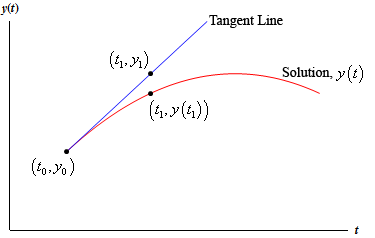
\includegraphics[width=0.8\textwidth]{euler_example.png}
	\caption{}
	\label{fig:euler_example}
\end{figure}

For this method it is quite straightforward to find stability conditions 
analytically. 
 
%%%%%%%%%%%%%%%%%%%%%%%%%%%%%%%%%%%%%%%%%%%%%%%%%%%%%%%%%%%%%%%%%%%%%
\begin{thebibliography}{20}

bibitem{euler_example}
Paul's Online Math Notes, 2012. [online] Available at \url{http://tutorial.math.lamar.edu/Classes/DE/EulersMethod.asp}
[Accessed 8 November 2012].

\end{thebibliography}

\end{document}

